\documentclass[12pt]{article}
\usepackage{graphicx} % Required for inserting images
\usepackage{geometry}
\usepackage{amsmath}
\usepackage{hyperref}
\usepackage{amsmath}
\usepackage{enumitem}
\usepackage{amsfonts}
\usepackage{amssymb}
\usepackage{graphicx}
\usepackage{hyperref}
\usepackage{listings}
\usepackage{xcolor}
\usepackage{titling}
\usepackage{amsmath}
\usepackage{amssymb}
\usepackage{listings}
\usepackage{url}
\usepackage{tikz}
\usepackage{subcaption}





\begin{document}

\title{Schur Numbers Week 7 Report}
\date{\today}
\begin{titlepage}
    \begin{center}
        \vspace*{1cm}

        \rule{\linewidth}{0.2mm} \\[0.4cm]
        {\Large \textbf{CSE 326 Analysis and Design of Algorithms }}\\[0.4cm]
        \textbf{Dr.Walid Gomaa}
 
        \rule{\linewidth}{0.2mm} \\[1.5cm]

        \begin{tabular}{c}
            \begin{tabular}{ll}
                \textbf{Name} & \textbf{ID} \\
                \hline
                Mohamed Abdelmonem Makram & 120220055 \\
                \hline
                Abdelrahman Ahmed Shaheen & 120220228 \\
                \hline
                Abdelrhman Mohamed Eldenary & 120220253 \\
                \hline
                Anas Ihab  Badr & 120220360 \\
                

            \end{tabular}
        \end{tabular}

        \vspace{1cm}

        

        \vspace{5cm}

        
\includegraphics[width=0.25\textwidth]{ejust.jpg}


        Computer Science Engineering Department\\
        Egypt-Japan University of Science and Technology\\

    \end{center}
\end{titlepage}


\tableofcontents
\newpage
\maketitle

\section{Recap}
In Week 5 we began to think about the idea of nested parallelism where we said we would use CUDA to try to brute force smartly enough where each thread
would call other threads to complete the problem. \\ 

In Week 6 we began to learn CUDA and its basics. We compiled a simple program that uses our two pointer algorithm to check for the available colorings of the next number, which would be the first step in the nested parallelism approach. As each nested thread will then have a version of the problem with the next number colored differently. \\ 

Currently, in Week 7 before implementing the nested parallelism approach, we would try to add another layer of randomness to the algorithm which we believe may help in getting results. We will explain this in the next section.

\section{Randomness}

Since our main goal is to try to improve the lower bound for $S(6)$, we would be working on the already existing coloring of $S(5)$. But as can be seen in the comparison between $S(4)$ and $S(3)$ in Figures \ref{fig:schur3}, \ref{fig:schur4} and  the original $S(3)$ coloring didn't persist in the $S(4)$ coloring. This implies that we cannot directly work on the $S(5)$ coloring, but we should choose one random number (at least) and change its coloring.

\begin{figure}[h!]
    \centering
    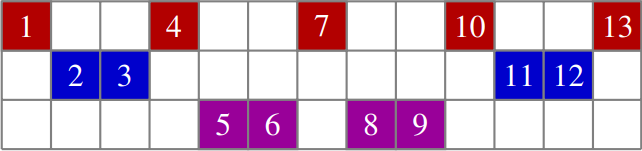
\includegraphics[width=0.5\textwidth]{schur_three.png}
    \caption{Schur Number 3 Coloring}
    \label{fig:schur3}
\end{figure}    

\vspace{1cm} % Adds vertical space between the images

\begin{figure}[h!]
    \centering
    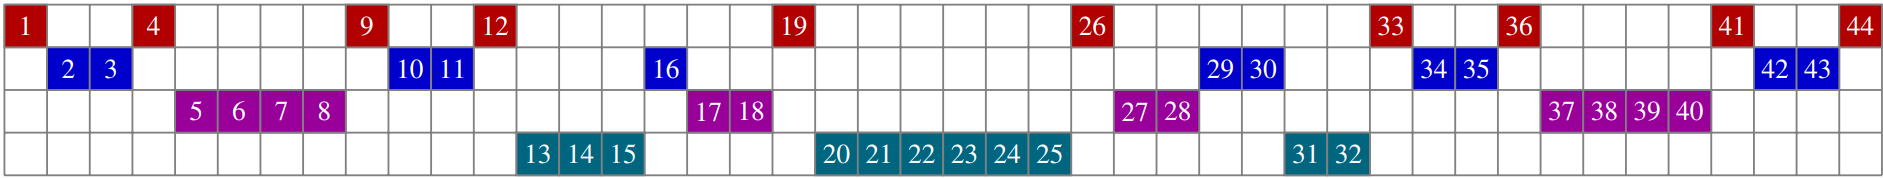
\includegraphics[width=\textwidth]{schur_four.png}
    \caption{Schur Number 4 Coloring}
    \label{fig:schur4}
\end{figure}

\subsection{Randomness in Coloring}
We would choose a random number and change its coloring. We designed an algorithm to test if changing number $x$ from coloring $A$ to coloring $B$ is valid or not. If it is valid, we would then continue with the new coloring in the nested parallelism approach. If it is not valid, we would choose another random number and repeat the process. We would repeat this process until we find a valid coloring.
The code for updating the coloring is included in the repository. The code takes as an input the amount of numbers that we wish to update its coloring randomly and return the updated coloring and how many steps it took to find a valid coloring.

\subsection{Results}
Here are the results of the recoloring of a coloring we made. We chose to recolor 1 number randomly. The results are as follows:

\begin{figure}
    \centering
    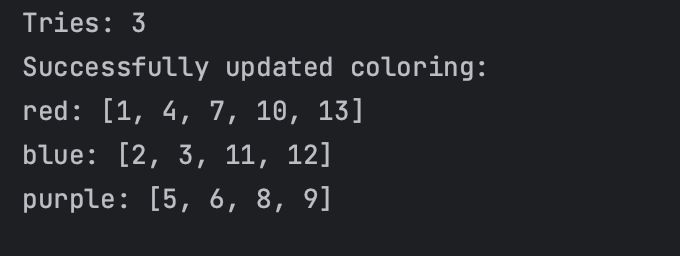
\includegraphics[width=\textwidth]{recoloring_results.jpeg}
    \caption{Recoloring Results}
    \label{fig:recoloring}
\end{figure}
    

\end{document}